\documentclass[../differential_methods.tex]{subfiles}
\begin{document}
\section{Aula 06 - 18 de Março, 2026}
\subsection{Motivações}
\begin{itemize}
	\item Esquema de diferenças centrais;
	\item Número de condições.
\end{itemize}
\subsection{Esquema de Diferenças Centrais e Acurácia}
Para dar procedência, precisamos lembrar o que fizemos na última aula: discretizamos o domínio usando uma malha cartesiana uniforme (uma coleção de pontos \((x_{j}, y_{j})\), onde \(x_{i}=i\Delta x\), \(y_{i}=j\Delta y\), e \(\Delta x\) e \(\Delta y\) são os tamanhos da malha nas direções x e y) e começamos a buscar nossas aproximações para \(u(x_{i}, y_{j})\), denotadas por \(U_{ij}\); note que temos \(n \times m\) como total, sendo m o tamanho da discretização em x e n da discretização em y.

Com o conhecimento de aproximação das derivadas e tendo em vista que desejamos encontrar \(U_{ij},\) consideramos também \(f_{ij}\coloneqq f(x_{i}, y_{j})\), a partir dos quais aplicamos o método de diferenças centrais à EDP:
\begin{align*}
	            & u_{xx}(x_{i}, y_{j})+u_{yy}(x_{i}, y_{j})=f(x_{i}, y_{j})                                                                             \\
	\Rightarrow & \frac{1}{(\Delta x)^{2}}[u(x_{i-1}, y_{j})-2u(x_{i}, y_{j})+u(x_{i+1}, y_{j})]                                                        \\
	+           & \frac{1}{(\Delta y)^{2}}[u(x_{i}, y_{j-1})-2u(x_{i}, y_{j})+u(x_{i}, y_{j+1})]+\mathcal{O}(\Delta x^{2}+\Delta y^{2})=f(x_{i}, y_{j}) \\
	\Rightarrow & \frac{1}{(\Delta x)^{2}}(U_{i-1, j}-2U_{ij}+U_{i+1, j})+\frac{1}{(\Delta y)^{2}}(U_{i, j-1}-2U_{ij}+ U_{i, j+1})=f_{ij},
\end{align*}
onde \(i=1,2,\dotsc ,m\) e \(j=1,2,\dotsc , n\). Por simplicidade, supusemos \(\Delta x = \Delta y = h\), resultando em uma aproximação centrada com 5 pontos da forma
\[
	\nabla_{5}^{2}U_{ij} \coloneqq \frac{1}{h^{2}}(U_{i-1, j}+U_{i+1, j}-4U_{ij}+U_{i+1, j}+U_{i, j+1})=f_{ij}.
\]

Consideremos as partições cartesianas \(0=x_{0}<x_1<\dotsc <x_{m}<x_{m+1}=1\) e \(0=y_{0}<y_1<\dotsc <y_{m}<y_{m+1}=1\), tais que \(h=\frac{1}{m+1}\).
Pelas equações acima, ganhamos um sistema linear de tamanho \(m^{2}\times m^{2}\) e forma \(A U = F\), com \(1\leq i\leq m,\; 1\leq j\leq m\), onde A é uma matriz esparsa:
\begin{figure}[H]
	\begin{center}
		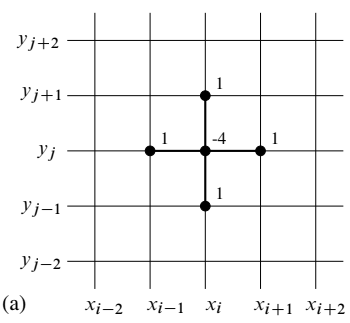
\includegraphics[height=0.35\textheight, width=0.35\textwidth, keepaspectratio]{./Images/five_stencil_05.png}
	\end{center}
	\caption{porção da malha computacional para a equação elíptica em duas dimensões. No exemplo, temos um estêncil de cinco pontos para o Laplaciano em torno de \((x_{i}, y_{j})\) com os pesos indicados.}
\end{figure}
Para a equação acima, podemos seguir um sentido de linhas para a escrita de cada termo da equação, com o auxílio visual da cruz, resultando nos termos
\begin{align*}
	 & U^{[j]}=\begin{bmatrix}
		           U_{1j} \\
		           U_{2j} \\
		           \vdots \\
		           U_{mj}
	           \end{bmatrix},\quad  U = \begin{bmatrix}
		                                    U^{[1]} \\
		                                    U^{[2]} \\
		                                    \vdots  \\
		                                    U^{[m]}
	                                    \end{bmatrix},                                  \\
	 & f^{[j]}=\begin{bmatrix}
		           f_{1j} \\
		           f_{2j} \\
		           \vdots \\
		           f_{mj}
	           \end{bmatrix}+BV, \quad F = \begin{bmatrix}
		                                       f^{[1]} \\
		                                       f^{[2]} \\
		                                       \vdots  \\
		                                       f^{[m]}
	                                       \end{bmatrix}                               \\
	 & T = \begin{bmatrix}
		       -4     & 1      & \dotsc &        &        \\
		       1      & -4     & 1      & \dotsc &        \\
		       \vdots & \ddots & \ddots & \ddots & \dotsc \\
		              &        & 1      & -4     & 1      \\
		              &        &        & 1      & -4
	       \end{bmatrix}_{\mathrlap{m\times m}},\quad A = \frac{1}{h^{2}}\begin{bmatrix}
		                                                                     T      & I      & \dotsc                   \\
		                                                                     I      & T      & I      & \dotsc          \\
		                                                                     \vdots & \ddots & \ddots & \ddots & \dotsc \\
		                                                                            &        & I      & T      & I      \\
		                                                                            &        &        & I      & T
	                                                                     \end{bmatrix}_{m^{2}\times m^{2}}
\end{align*}
onde \(I\in \mathbb{R}^{m\times m}\) é uma matriz identidade. Note que, ao construir a matriz T, os lugares onde os índices são i e j, correspondentes exatamente à diagonal, ficaram com 4 (o termo \(-4U_{ij}\) tem coeficiente -4, com entradas ij), e nos termos conde i ou j diferem por \(\pm1\), as entradas foram 1 (analogamente, \(U_{i-1, j},\; U_{i+1, j},\; U_{i, j-1}\) e \(U_{i, j+1}\) são todos acompanhados por coeficiente 1); caso contrário, como todo o resto foi zerado na aproximação, é tudo 0. Tendo montado a matriz T, a A segue basicamente da montagem em blocos.
\begin{exr}
	Generalize a definição de A utilizando uma malha \(m\times n\) para discretizar o domínio \(\Omega \), e utilize o \hyperlink{kronecker_matrix}{\textit{produto matricial de Kronecker}} para construir a matriz A (no MATLAB, é o comando \texttt{kron}). Uma dcia é que a forma final será
	\[
		T\otimes I + I\otimes \begin{bmatrix}
			0      & 1      & \dotsc &        \\
			1      & 0      & 1      & \dotsc \\
			\vdots & \ddots & \ddots & \dotsc \\
			       &        & 1      & 0
		\end{bmatrix}
	\]. Por fim, escreva a forma final de BV na definição de F.
\end{exr}
\begin{figure}[H]
	\begin{center}
		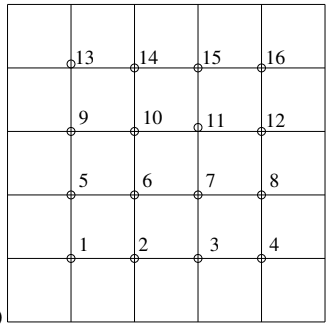
\includegraphics[height=0.35\textheight, width=0.35\textwidth, keepaspectratio]{./Images/row_wise_05.png}
	\end{center}
	\caption{a ordem natural de incógnitas no sentido das linhas em uma grade 4x4; os nós externos podem ser vistos como fronteiras de Dirichlet!}
\end{figure}
\begin{tcolorbox}[
		skin=enhanced,
		title=Lembrete!,
		after title={\hfill Produto Matricial de Kronecker},
		fonttitle=\bfseries,
		sharp corners=downhill,
		colframe=black,
		colbacktitle=yellow!75!white,
		colback=yellow!30,
		colbacklower=black,
		coltitle=black,
		%drop fuzzy shadow,
		drop large lifted shadow
	]
	O \hypertarget{kronecker_matrix}{\textbf{produto matricial de Fornecer}} entre matrizes A, de tamanho \(m\times n\), e B, de tamanho \(p\times q\), é uma matriz de tamanho \(pm \times qn\) em blocos, dado por
	\begin{align*}
		 & A \otimes B = \begin{bmatrix}
			                 a_{11}B & \dotsc & a_{1n}B \\
			                 \vdots  & \ddots & \vdots  \\
			                 a_{m1}B & \dotsc & a_{mn}B
		                 \end{bmatrix}                                                                                      \\
		 & = \begin{bmatrix}
			     a_{11}b_{11} & a_{11}b_{12} & \dotsc & a_{11}b_{1q} & \dotsc & \dotsc & a_{1n}b_{11} & a_{1n}b_{12} & \dotsc & a_{1n}b_{1q} \\
			     a_{11}b_{21} & a_{11}b_{22} & \dotsc & a_{11}b_{2q} & \dotsc & \dotsc & a_{1n}b_{21} & a_{1n}b_{22} & \dotsc & a_{1n}b_{2q} \\
			     \vdots       & \vdots       & \ddots & \vdots       & \ddots & \ddots & \ddots       & \vdots       & \ddots & \vdots       \\
			     a_{11}b_{p1} & a_{11}b_{p2} & \dotsc & a_{11}b_{pq} & \dotsc & \dotsc & a_{1n}b_{p1} & a_{1n}b_{p2} & \dotsc & a_{1n}b_{pq} \\
			     \vdots       & \vdots       & \ddots & \vdots       & \ddots & \ddots & \ddots       & \vdots       & \ddots & \vdots       \\
			     \vdots       & \vdots       & \ddots & \vdots       & \ddots & \ddots & \ddots       & \vdots       & \ddots & \vdots       \\
			     a_{m1}b_{11} & a_{m1}b_{12} & \dotsc & a_{m1}b_{1q} & \dotsc & \dotsc & a_{mn}b_{11} & a_{mn}b_{12} & \dotsc & a_{mn}b_{1q} \\
			     \vdots       & \vdots       & \ddots & \vdots       & \ddots & \ddots & \ddots       & \ddots       & \vdots & \vdots       \\
			     a_{m1}b_{p1} & a_{m1}b_{p2} & \dotsc & a_{m1}b_{pq} & \dotsc & \dotsc & a_{mn}b_{p1} & a_{mn}b_{p2} & \dotsc & a_{mn}b_{pq} \\
		     \end{bmatrix}
	\end{align*}
	Esse produto é bilinear, associativo, não comutativo e satisfaz
	\[
		(A\otimes B)(C\otimes D)=(AC)\otimes (BD),\quad (A\otimes B)^{T}=A^{T}\otimes B^{T}.
	\]
\end{tcolorbox}

O erro de truncamento local \(\tau_{ij}\) em um ponto \((i, j)\) da malha é dado por
\[
	\tau_{ij}\coloneqq \frac{1}{h^{2}}(u(x_{i-1}, y_{j})+u(x_{i+1}, y_{j})+u(x_{i}, y_{j-1})+u(x_{i}, y_{j+1})-4u(x_{i}, y_{j}))-f(x_{i}, y_{j}),
\]
que podemos expandir em Taylor para obter
\[
	\tau_{ij}\coloneqq \frac{1}{12}h^{2}(\partial_{x}^{(4)}u(x_{i}, y_{j})+\partial_{y}^{(4)}u(x_{i}, y_{j}))+\mathcal{O}(h^{4}),
\]
tal que, colocando \(\hat{U}=(u(x_1,y_1), \dotsc , u(x_{m}, y_{m}))^{T}\in \mathbb{R}^{m^{2}}\), obtemos
\[
	A \hat{U}=F+\tau ,
\]
onde A é a matriz de discretização segundo a ordenação com respeito às linhas.

Denotando por \(E_{ij}\coloneqq U_{ij}-u(x_{i}, y_{j})\) o erro global e observando que \(AU=F\), temos a relação
\[
	AE=-\tau \Rightarrow E=A^{-1}(-\tau )\Rightarrow \Vert E \Vert\leq \Vert A^{-1} \Vert\Vert \tau  \Vert.
\]
Logo, caso \(\Vert A^{-1} \Vert\) seja uniformemente limitada\footnote{Lembrando que o tamanho de A é uma função do tamanho h da grade.} conforme h tende a zero, segue que esse método garante um erro global com acurácia de segunda ordem para algumas normas de funções em malhas.

É importante destacar que as definições de consistência, estabilidade e convergência continuam todas válidas no contexto da análise de métodos numéricos para equações elípticas.

Assim como antes, vamos ver a questão dos autovalores, autovetores e autofunções: consideremos uma 2-norma para a matriz de discretização A; fazendo umas contas, é possível mostrar que, para cada \(p, q=1,2,\dotsc ,m\), o autovetor \(u^{p, q}\) tem \(m^{2}\) entradas, dadas por
\[
	u_{ij}^{p, q}=\sin^{}{(p\pi ih)}\sin^{}{(q\pi jh)},
\]
com autovalores correspondentes
\[
	\lambda_{p,q}=\frac{2}{h^{2}}(\cos^{}{(p\pi h)}-1+\cos^{}{(q\pi h)}-1)<0, \quad h=\frac{1}{m+1}.
\]
Assim, o autovalor mais próximo à origem é \(\lambda_{1,1}=-2\pi^{2}+\mathcal{O}(h^{2})\) por meio das expansões de Taylor. Quanto às características resultantes disso, o raio espectral de \(A^{-1}\) é dado por
\[
	\pi (A^{-1})=\frac{1}{| \lambda_{1,1} |}\leq \frac{1}{2\pi^{2}},\quad h\to 0^{+},
\]
de modo que sua 2-norma tenha também um limite uniforme conforme \(h\to 0^{+}\):
\begin{align*}
	\Vert A^{-1} \Vert_{2}=\sqrt[]{\rho (A^{-T}A^{-1})} & = \sqrt[]{\rho((A^{-1})^{2})}  \\
	                                                    & = \sqrt[]{\rho ((A^{-1})^{2})} \\
	                                                    & = \rho (A^{-1})                \\
	                                                    & \leq \frac{1}{2\pi^{2}}.
\end{align*}

\begin{tcolorbox}[
		skin=enhanced,
		title=Observação,
		fonttitle=\bfseries,
		colframe=black,
		colbacktitle=cyan!75!white,
		colback=cyan!15,
		colbacklower=black,
		coltitle=black,
		drop fuzzy shadow,
		%drop large lifted shadow
	]
	A numeração que fizemos foi por linha, como já dito; caso fosse feita por coluna, seria necessário inverter o papel do m e do n para todos os raciocínios!
\end{tcolorbox}

Note que a definição de estabilidade garante, também, a estabilidade de sistemas lineares que originem da discretização! De fato, considere o sistema discreto
\[
	AU = F,
\]
todos dependendo do tamanho h da malha. Suponha que causamos uma perturbação por um vetor pequeno p (\(\Vert p \Vert_{2}<0\) para algum \( \delta >0\) pequeno) ao lado direito da equação, e que a solução correspondente ao sistema perturbado é \(\hat{U}\). Então, neste contexto, temos
\[
	A\hat{U} = F +p,\; A U = F \Rightarrow A(\hat{U}-U)=F+p-F = p,
\]
tal que
\[
	\hat{U}-U=A^{-1}p \Rightarrow \Vert \hat{U}-U \Vert_{2}\leq \Vert A^{-1} \Vert_{2}\Vert p \Vert_{2}.
\]
Porém, por hipótese, a perturbação foi menor que certo \(\delta > 0\) pequeno, permitindo relacionarmos
\[
	\Vert \hat{U}-U \Vert_{2}\leq \Vert A^{-1} \Vert_{2}\Vert p \Vert_{2}<\Vert A^{-1} \Vert_{2}\delta <C\delta ,
\]
garantindo a estabilidade para pequenas perturbações! (Tenha em mente que \(\Vert \hat{U}-U \Vert\) e \(\Vert p \Vert_{2}\) são ambas normas de funções nas malhas).

Nessa perspectiva de estimarmos a norma de A, tem uma definição útil:
\begin{def*}
	O \textbf{número de condição} da matriz A com respeito a uma norma matricial \(\Vert \cdot  \Vert\) é definido como
	\[
		\kappa (A)\coloneqq \Vert A \Vert\Vert A^{-1} \Vert. \; \square
	\]
\end{def*}
O número de condição é uma medida do quanto o valor final da matriz mudará para pequenas perturbações, ou seja, ele dá uma noção de limite da imprecisão do resultado após uma aproximação. Por exemplo, vamos considerar a norma \(\Vert \cdot  \Vert_{2}\); note que, conforme \(h\to 0^{+}\), temos
\begin{align*}
	\Vert A \Vert_{2} = \rho (A) & = \max\limits_{1\leq p, q\leq }| \lambda_{p, q} |                                   \\
	                             & = | \lambda_{m, m} |                                                                \\
	                             & = \frac{4}{h^{2}}\biggl\vert \cos^{}{\biggl(\frac{m}{m+1}\pi \biggr)} -1\biggr\vert \\
	                             & \approx \frac{4}{h^{2}}| -2 |                                                       \\
	                             & = \frac{8}{h^{2}}.
\end{align*}
Portanto, tendo em vista que determinamos anteriormente a aproximação \(\Vert A^{-1} \Vert\approx \frac{1}{2\pi^{2}},\) vale que
\[
	\kappa (A)\approx \frac{8}{h^{2}}\frac{1}{2\pi^{2}}=\frac{4}{\pi^{2}h^{2}}=\mathcal{O}(h^{-2}),
\]
e podemos concluir que a matriz de discretização A é mal-comportada cada vez que refinamos a malha, já que \(\kappa (A)\) cresce quadraticamente ao infinito conforme h diminui.

Na próxima aula, vamos brincar com a reordenação do que fizemos hoje e discutir um pouco das condições de Neumann: imagine que o contorno passa a ser um contorno de Neumann ao invés de Dirichlet, condicionando não apenas em u, mas também no gradiente de u!
\end{document}
